\section{Convenios de pago}


Financiación de deuda contractual, cuotas y efectos de pagos relacionados.


\begin{quote}
\textbf{Ficha de dominio:} documenta convenios, cuotas, resumen de deuda y pagos relacionados, incluidos sus estados, efectos derivados y superficies de generación de PDF.
\end{quote}


\subsection{Alcance y entradas HTTP}


\begin{itemize}
\item \textbf{Controladores:} \texttt{\detokenize{AgreementsController}} y, para pagos que afectan cuotas, \texttt{\detokenize{PaymentsController}}.
\item \textbf{Servicios:} \texttt{\detokenize{AgreementsService}} y \texttt{\detokenize{PaymentsService}}.
\item \textbf{Casos:} \texttt{\detokenize{GetDebtSummaryUseCase}}, \texttt{\detokenize{CreateAgreementUseCase}}, \texttt{\detokenize{FindOneAgreementUseCase}}, \texttt{\detokenize{UpdateAgreementUseCase}}, \texttt{\detokenize{GetPaymentAgreementPdfDataUseCase}}, \texttt{\detokenize{CreatePaymentUseCase}}, \texttt{\detokenize{ValidatePaymentUseCase}}, \texttt{\detokenize{AnnulPaymentUseCase}}, \texttt{\detokenize{ApplySaldoFavorUseCase}}.
\item Listar convenios y catálogos se resuelven directamente en los servicios; no se confirmó caso dedicado para \texttt{\detokenize{findAll}} ni para catálogos.
\end{itemize}


\begin{center}
\small
\begin{longtable}{|p{0.313\textwidth}|p{0.313\textwidth}|p{0.313\textwidth}|}
\hline
\textbf{Método y ruta} & \textbf{Caso/servicio ejecutado} & \textbf{Resultado} \\
\hline
\endfirsthead
\hline
\textbf{Método y ruta} & \textbf{Caso/servicio ejecutado} & \textbf{Resultado} \\
\hline
\endhead
\texttt{\detokenize{GET /api/v1/agreements/states}} & \texttt{\detokenize{findAllAgreementStates()}} & Estados de convenio. \\
\hline
\texttt{\detokenize{GET /api/v1/agreements/installment-states}} & \texttt{\detokenize{findAllInstallmentStates()}} & Estados de cuota. \\
\hline
\texttt{\detokenize{GET /api/v1/agreements/debt-summary/:contratoId}} & \texttt{\detokenize{getDebtSummary()}} → \texttt{\detokenize{GetDebtSummaryUseCase}} & Deuda. \\
\hline
\texttt{\detokenize{POST /api/v1/agreements}} & \texttt{\detokenize{create()}} → \texttt{\detokenize{CreateAgreementUseCase}} & Convenio y cuotas. \\
\hline
\texttt{\detokenize{GET /api/v1/agreements}} / \texttt{\detokenize{:id}} / \texttt{\detokenize{:id/installments}} & servicio / \texttt{\detokenize{FindOneAgreementUseCase}} & Convenio/cuotas. \\
\hline
\texttt{\detokenize{PATCH /api/v1/agreements/:id}} & \texttt{\detokenize{update()}} → \texttt{\detokenize{UpdateAgreementUseCase}} & Estado. \\
\hline
\texttt{\detokenize{DELETE /api/v1/agreements/:id}} & \texttt{\detokenize{cancel()}} → \texttt{\detokenize{UpdateAgreementUseCase(ANULADO)}} & Anulación. \\
\hline
\texttt{\detokenize{GET /api/v1/agreements/:id/pdf}} & \texttt{\detokenize{generatePdf()}} → \texttt{\detokenize{GetPaymentAgreementPdfDataUseCase}} & PDF. \\
\hline
\texttt{\detokenize{POST/PATCH/DELETE /api/v1/payments...}} & casos de pagos & Crea, valida, aplica o anula pagos. \\
\hline
\end{longtable}
\end{center}


\subsection{Ejemplo JSON}


\begin{lstlisting}
{
  "convenioId": "8",
  "contratoId": "1",
  "deudaTotal": 240.5,
  "abonoInicial": 40,
  "numeroCuotas": 5,
  "estado": "PENDIENTE_ABONO",
  "cuotas": [
    {
      "cuotaConvenioId": "81",
      "numeroCuota": 1,
      "valorCuota": 40.1,
      "estado": "PENDIENTE"
    }
  ]
}
\end{lstlisting}


\begin{center}
\small
\begin{longtable}{|p{0.313\textwidth}|p{0.313\textwidth}|p{0.313\textwidth}|}
\hline
\textbf{Campo} & \textbf{Tipo} & \textbf{Regla/uso} \\
\hline
\endfirsthead
\hline
\textbf{Campo} & \textbf{Tipo} & \textbf{Regla/uso} \\
\hline
\endhead
\texttt{\detokenize{convenioId}}, \texttt{\detokenize{contratoId}}, \texttt{\detokenize{cuotaConvenioId}} & string & \texttt{\detokenize{BigInt}} serializado. \\
\hline
\texttt{\detokenize{deudaTotal}}, \texttt{\detokenize{abonoInicial}}, \texttt{\detokenize{valorCuota}} & number & Valores monetarios. \\
\hline
\texttt{\detokenize{numeroCuotas}}, \texttt{\detokenize{numeroCuota}} & number & Plan y posición. \\
\hline
\texttt{\detokenize{estado}} & enum & Estado de convenio o cuota según el objeto. \\
\hline
\end{longtable}
\end{center}


\subsection{Estados}


\begin{center}
\small
\begin{longtable}{|p{0.313\textwidth}|p{0.313\textwidth}|p{0.313\textwidth}|}
\hline
\textbf{Entidad} & \textbf{Estados} & \textbf{Significado} \\
\hline
\endfirsthead
\hline
\textbf{Entidad} & \textbf{Estados} & \textbf{Significado} \\
\hline
\endhead
Convenio & \texttt{\detokenize{PREPARADO}}, \texttt{\detokenize{PENDIENTE_ABONO}}, \texttt{\detokenize{ACTIVO}}, \texttt{\detokenize{PAGADO}}, \texttt{\detokenize{ANULADO}} & Creado, abono pendiente, vigente, liquidado o anulado. \\
\hline
Cuota & \texttt{\detokenize{PENDIENTE}}, \texttt{\detokenize{PAGADA}} & No liquidada o liquidada. \\
\hline
Pago relacionado & \texttt{\detokenize{PENDIENTE}}, \texttt{\detokenize{REGISTRADO}}, \texttt{\detokenize{ANULADO}} & Por validar, validado o anulado. \\
\hline
\end{longtable}
\end{center}


\subsection{Efectos y transacciones}


Crear convenio calcula deuda y cuotas y persiste \texttt{\detokenize{Convenios}}/\texttt{\detokenize{CuotaConvenio}} en transacción. \texttt{PagoValidadoHandler} actualiza prefacturas y contratos de instalación; \texttt{CuotaPagadaHandler} verifica cuotas y dispara emisión SRI. \texttt{PagoAnuladoHandler} emite nota de crédito si corresponde; no se confirmó rollback de cuotas, prefacturas o contratos. La generación de catálogos, consultas y DTO es pura.

\subsubsection{Tablas y fórmulas confirmadas}
La relación es \texttt{Contratos $\rightarrow$ Convenios $\rightarrow$ CuotaConvenio $\rightarrow$ PrefacturaDetalle $\rightarrow$ Prefacturas}. La deuda usa prefacturas no eliminadas en estados \texttt{GENERADA}, \texttt{EN\_REVISION} o \texttt{APROBADA}:
\[
\text{saldoPrefactura}=\max(0,\text{totalPagar}-\text{abono}),\quad
\text{deudaTotal}=\operatorname{ROUND\_HALF\_UP}(\sum\text{saldoPrefactura},2).
\]
\texttt{mesesMoraActual} cuenta saldos positivos y \texttt{deudaAnterior} busca el período inmediatamente anterior; la continuidad de períodos es una limitación. Fuentes: \texttt{backend/src/billing/collections/agreements/application/use-cases/get-debt-summary.use-case.ts}, \texttt{prisma-agreement-repository.ts} y \texttt{backend/src/shared/utils/debt-calculator.util.ts}.

La tasa se normaliza como \texttt{tasaMensual=tasa/100}; el interés lineal es
\[
\text{interés}=(\text{deudaTotal}-\text{abonoInicial})\times\text{tasaMensual}\times\text{numeroCuotas},\quad
\text{totalADistribuir}=\text{deudaTotal}-\text{abonoInicial}+\text{interés}.
\]
La cuota base es \texttt{TRUNC(totalADistribuir/numeroCuotas,2)} y la última absorbe el residuo. \texttt{CreateAgreementUseCase} (aprox. líneas 30--220) valida deuda, abono, cuotas, tasa y transiciones en transacción. El vencimiento es mensual desde la fecha base.


\begin{center}
\small
\begin{longtable}{|p{0.470\textwidth}|p{0.470\textwidth}|}
\hline
\textbf{Tabla Prisma} & \textbf{Uso} \\
\hline
\endfirsthead
\hline
\textbf{Tabla Prisma} & \textbf{Uso} \\
\hline
\endhead
\texttt{\detokenize{Convenios}} & Plan y estado. \\
\hline
\texttt{\detokenize{CuotaConvenio}} & Cuotas y pagos aplicados. \\
\hline
\texttt{\detokenize{Contratos}}, \texttt{\detokenize{Prefacturas}}, \texttt{\detokenize{PrefacturaDetalle}}, \texttt{\detokenize{Rubros}} & Deuda de origen. \\
\hline
\texttt{\detokenize{Pagos}}, \texttt{\detokenize{DetallePago}}, \texttt{\detokenize{SaldoFavor}} & Cobros y saldos. \\
\hline
\end{longtable}
\end{center}


\subsection{Gráfico de estados}


\begin{lstlisting}
stateDiagram-v2
  [*] --> PREPARADO
  PREPARADO --> PENDIENTE_ABONO
  PENDIENTE_ABONO --> ACTIVO: abono validado
  ACTIVO --> PAGADO: cuotas liquidadas
  ACTIVO --> ANULADO
\end{lstlisting}


\subsection{Casos de uso}


\subsubsection{Caso: Consultar estados de convenio}


\textbf{Descripción:} entrega el catálogo de estados disponibles para convenios.  

\textbf{HTTP y ruta:} \texttt{\detokenize{GET /api/v1/agreements/states}}.  

\textbf{Permiso:} \texttt{\detokenize{agreements:read}}.  

\textbf{Cadena:} \texttt{\detokenize{AgreementsController.findAllStates()}} → \texttt{\detokenize{AgreementsService.findAllAgreementStates()}} → enum.  

\textbf{Errores relevantes:} \texttt{\detokenize{401}}; \texttt{\detokenize{403}}.  

\textbf{Efectos:} ninguno; catálogo de lectura.  

\textbf{Prisma:} ninguna tabla.  

\textbf{Entrada:} sin body, path ni query.  

\textbf{Salida:} \texttt{\detokenize{[ { "codigo": "ACTIVO", "descripcion": "Activo" } ]}}.


\subsubsection{Caso: Consultar estados de cuota}


\textbf{Descripción:} entrega el catálogo de estados disponibles para cuotas.  

\textbf{HTTP y ruta:} \texttt{\detokenize{GET /api/v1/agreements/installment-states}}.  

\textbf{Permiso:} \texttt{\detokenize{agreements:read}}.  

\textbf{Cadena:} \texttt{\detokenize{AgreementsController.findAllInstallmentStates()}} → \texttt{\detokenize{AgreementsService.findAllInstallmentStates()}} → enum.  

\textbf{Errores relevantes:} \texttt{\detokenize{401}}; \texttt{\detokenize{403}}.  

\textbf{Efectos:} ninguno; catálogo de lectura.  

\textbf{Prisma:} ninguna tabla.  

\textbf{Entrada:} sin body, path ni query.  

\textbf{Salida:} \texttt{\detokenize{[ { "codigo": "PENDIENTE", "descripcion": "Pendiente" } ]}}.


\subsubsection{Caso: Consultar resumen de deuda}


\textbf{Descripción:} calcula el resumen de deuda pendiente y devuelve el detalle de las prefacturas impagadas. No expone un total agregado \texttt{montoPagado} en este caso de uso.  

\textbf{HTTP y ruta:} \texttt{\detokenize{GET /api/v1/agreements/debt-summary/:contratoId}}.  

\textbf{Permiso:} \texttt{\detokenize{agreements:read}}.  

\textbf{Cadena:} \texttt{\detokenize{AgreementsController.getDebtSummary()}} → \texttt{\detokenize{AgreementsService.getDebtSummary()}} → \texttt{\detokenize{GetDebtSummaryUseCase.execute()}} → repositorio.  

\textbf{Errores relevantes:} \texttt{\detokenize{400}}; \texttt{\detokenize{401}}; \texttt{\detokenize{403}}; \texttt{\detokenize{404}}.  

\textbf{Efectos:} ninguno.  

\textbf{Prisma:} \texttt{\detokenize{Contratos}}, \texttt{\detokenize{Prefacturas}}, \texttt{\detokenize{PrefacturaDetalle}}, \texttt{\detokenize{Rubros}}, pagos.  

\textbf{Entrada:} sin body; path \texttt{\detokenize{{ "contratoId": "1" }}}.  

\textbf{Salida:} \texttt{\detokenize{{ "contratoId": "1", "deudaTotal": 240.5, "deudaAnterior": 40, "tasaMensualVigente": 2.5, "maxMesesAtrasado": 2, "totalPrefacturasImpagadas": 3, "prefacturas": [] }}}.


\subsubsection{Caso: Crear convenio}


\textbf{Descripción:} crea un plan de pago y genera sus cuotas.  

\textbf{HTTP y ruta:} \texttt{\detokenize{POST /api/v1/agreements}}.  

\textbf{Permiso:} \texttt{\detokenize{agreements:create}}.  

\textbf{Cadena:} \texttt{\detokenize{AgreementsController.create()}} → \texttt{\detokenize{AgreementsService.create()}} → \texttt{\detokenize{CreateAgreementUseCase.execute()}} → repositorio.  

\textbf{Errores relevantes:} \texttt{\detokenize{400}}; \texttt{\detokenize{401}}; \texttt{\detokenize{403}}; \texttt{\detokenize{404}}; deuda no convenible.  

\textbf{Efectos:} persiste convenio y cuotas; no activa por sí solo el contrato.  

\textbf{Prisma:} \texttt{\detokenize{Convenios}}, \texttt{\detokenize{CuotaConvenio}}, \texttt{\detokenize{Contratos}}, prefacturas/rubros.  

\textbf{Entrada:} \texttt{\detokenize{{ "contratoId": "1", "abonoInicial": 40, "numeroCuotas": 5 }}}.  

\textbf{Salida:} JSON del ejemplo principal.


\subsubsection{Caso: Listar convenios}


\textbf{Descripción:} lista convenios paginados y filtrables.  

\textbf{HTTP y ruta:} \texttt{\detokenize{GET /api/v1/agreements}}.  

\textbf{Permiso:} \texttt{\detokenize{agreements:read}}.  

\textbf{Cadena:} \texttt{\detokenize{AgreementsController.findAll()}} → \texttt{\detokenize{AgreementsService.findAll()}} → repositorio; sin caso dedicado confirmado.  

\textbf{Errores relevantes:} \texttt{\detokenize{400}}; \texttt{\detokenize{401}}; \texttt{\detokenize{403}}.  

\textbf{Efectos:} ninguno.  

\textbf{Prisma:} \texttt{\detokenize{Convenios}}, contrato/cliente.  

\textbf{Entrada:} sin body; query \texttt{\detokenize{page}}, \texttt{\detokenize{limit}}, \texttt{\detokenize{contratoId}}, \texttt{\detokenize{estado}}, \texttt{\detokenize{search}}.  

\textbf{Salida:} \texttt{\detokenize{{ "data": [{ "convenioId": "8", "estado": "ACTIVO" }], "meta": {} }}}.


\subsubsection{Caso: Obtener convenio}


\textbf{Descripción:} devuelve el detalle de un convenio por identificador.  

\textbf{HTTP y ruta:} \texttt{\detokenize{GET /api/v1/agreements/:id}}.  

\textbf{Permiso:} \texttt{\detokenize{agreements:read}}.  

\textbf{Cadena:} \texttt{\detokenize{AgreementsController.findOne()}} → \texttt{\detokenize{AgreementsService.findOne()}} → \texttt{\detokenize{FindOneAgreementUseCase.execute()}} → repositorio.  

\textbf{Errores relevantes:} \texttt{\detokenize{400}}; \texttt{\detokenize{401}}; \texttt{\detokenize{403}}; \texttt{\detokenize{404}}.  

\textbf{Efectos:} ninguno; consulta y DTO puros.  

\textbf{Prisma:} \texttt{\detokenize{Convenios}}, \texttt{\detokenize{Contratos}}, \texttt{\detokenize{Clientes}}, \texttt{\detokenize{CuotaConvenio}}.  

\textbf{Entrada:} sin body; path \texttt{\detokenize{{ "id": "8" }}}.  

\textbf{Salida:} objeto JSON \texttt{\detokenize{AgreementResponseDto}} con sus datos y cuotas.


\subsubsection{Caso: Listar cuotas de un convenio}


\textbf{Descripción:} devuelve las cuotas asociadas a un convenio.  

\textbf{HTTP y ruta:} \texttt{\detokenize{GET /api/v1/agreements/:id/installments}}.  

\textbf{Permiso:} \texttt{\detokenize{agreements:read}}.  

\textbf{Cadena:} \texttt{\detokenize{AgreementsController.findInstallments()}} → \texttt{\detokenize{AgreementsService.findInstallments()}} → repositorio.  

\textbf{Errores relevantes:} \texttt{\detokenize{400}}; \texttt{\detokenize{401}}; \texttt{\detokenize{403}}; \texttt{\detokenize{404}}.  

\textbf{Efectos:} ninguno; consulta y DTO puros.  

\textbf{Prisma:} \texttt{\detokenize{CuotaConvenio}}, \texttt{\detokenize{Convenios}}.  

\textbf{Entrada:} sin body; path \texttt{\detokenize{{ "id": "8" }}}.  

\textbf{Salida:} lista JSON \texttt{\detokenize{[ { "cuotaConvenioId": "81", "numeroCuota": 1, "estado": "PENDIENTE" } ]}}.


\subsubsection{Caso: Actualizar estado del convenio}


\textbf{Descripción:} aprueba, paga o cambia el estado permitido del convenio.  

\textbf{HTTP y ruta:} \texttt{\detokenize{PATCH /api/v1/agreements/:id}}.  

\textbf{Permiso:} \texttt{\detokenize{agreements:update}}.  

\textbf{Cadena:} \texttt{\detokenize{AgreementsController.update()}} → \texttt{\detokenize{AgreementsService.update()}} → \texttt{\detokenize{UpdateAgreementUseCase.execute()}} → repositorio.  

\textbf{Errores relevantes:} \texttt{\detokenize{400}}; \texttt{\detokenize{401}}; \texttt{\detokenize{403}}; \texttt{\detokenize{404}}; transición inválida.  

\textbf{Efectos:} \texttt{\detokenize{PAGADO}} puede marcar convenio y cuotas.  

\textbf{Prisma:} \texttt{\detokenize{Convenios}}, \texttt{\detokenize{CuotaConvenio}}.  

\textbf{Entrada:} path \texttt{\detokenize{{ "id": "8" }}}; body \texttt{\detokenize{{ "estado": "ACTIVO" }}}.  

\textbf{Salida:} \texttt{\detokenize{{ "convenioId": "8", "estado": "ACTIVO" }}}.


\subsubsection{Caso: Anular convenio}


\textbf{Descripción:} marca un convenio como \texttt{\detokenize{ANULADO}}.  

\textbf{HTTP y ruta:} \texttt{\detokenize{DELETE /api/v1/agreements/:id}}.  

\textbf{Permiso:} \texttt{\detokenize{agreements:delete}}.  

\textbf{Cadena:} \texttt{\detokenize{AgreementsController.cancel()}} → \texttt{\detokenize{AgreementsService.cancel()}} → \texttt{\detokenize{UpdateAgreementUseCase(ANULADO)}}.  

\textbf{Errores relevantes:} \texttt{\detokenize{400}}; \texttt{\detokenize{401}}; \texttt{\detokenize{403}}; \texttt{\detokenize{404}}.  

\textbf{Efectos:} persiste anulación; no se confirma borrado físico.  

\textbf{Prisma:} \texttt{\detokenize{Convenios}}, cuotas si la transición las afecta.  

\textbf{Entrada:} sin body; path \texttt{\detokenize{{ "id": "8" }}}.  

\textbf{Salida:} \texttt{\detokenize{{ "convenioId": "8", "estado": "ANULADO" }}}.


\subsubsection{Caso: Generar PDF del convenio}


\textbf{Descripción:} genera el documento imprimible del plan.  

\textbf{HTTP y ruta:} \texttt{\detokenize{GET /api/v1/agreements/:id/pdf}}.  

\textbf{Permiso:} \texttt{\detokenize{agreements:read}}.  

\textbf{Cadena:} \texttt{\detokenize{AgreementsController.generatePdf()}} → \texttt{\detokenize{AgreementsService.generatePdf()}} → \texttt{\detokenize{GetPaymentAgreementPdfDataUseCase.execute()}} → dispatcher.  

\textbf{Errores relevantes:} \texttt{\detokenize{400}}; \texttt{\detokenize{401}}; \texttt{\detokenize{403}}; \texttt{\detokenize{404}}; aborto de solicitud.  

\textbf{Efectos:} sólo lectura y proyección; PDF puro.  

\textbf{Prisma:} \texttt{\detokenize{Convenios}}, \texttt{\detokenize{CuotaConvenio}}, \texttt{\detokenize{Contratos}}, \texttt{\detokenize{Clientes}}.  

\textbf{Entrada:} sin body; path \texttt{\detokenize{{ "id": "8" }}}.  

\textbf{Salida:} no es JSON: \texttt{\detokenize{application/pdf}}, \texttt{\detokenize{Content-Disposition: inline}}, \texttt{\detokenize{Content-Length}} y bytes PDF.


\subsection{No documentado o pendiente de confirmar}

\begin{figure}[h]
\centering
\IfFileExists{images/03-convenio-pago.png}{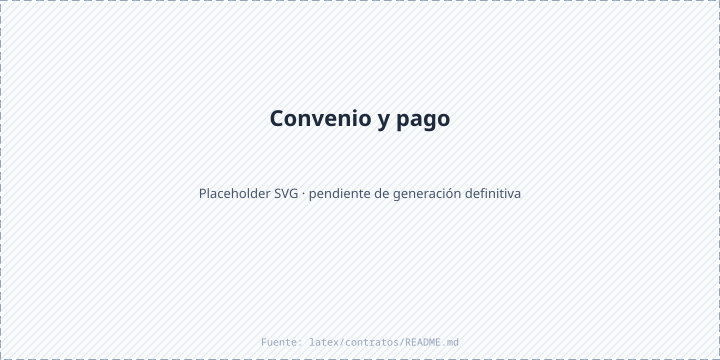
\includegraphics[width=0.9\textwidth]{images/03-convenio-pago.png}}{\fbox{\parbox{0.82\textwidth}{\centering Fallback: deuda $\rightarrow$ convenio $\rightarrow$ cuotas $\rightarrow$ pago. Agregar \texttt{images/03-convenio-pago.png} para reemplazarlo.}}}
\caption{Convenio y pago.}
\end{figure}


\begin{itemize}
\item No se encontró una política completa de mora ni una transición automática adicional fuera de los handlers documentados.
\item El registro de handlers está en \texttt{backend/src/billing/collections/payments/payments.module.ts} (aprox. líneas 1--180).
\item Umbral que convierte una cuota vencida en causal automática de corte.
\end{itemize}
